%----------------------------------------------------------------------------------------
%	SECTION 1.1
%----------------------------------------------------------------------------------------

\section{Topological Spaces.}

\begin{definition}
    A \textbf{topology} on a set $X$ is a collection  $\Tc$ of subsets of  $X$ such that: 
        \begin{enumerate}[label=(\arabic*)]
            \item $\emptyset, X \in \Tc$.

            \item For any subcollection $\{U_{\alpha}\}$ of subsets of $X$,  $\bigcup_{\alpha}{U_{\alpha}} \in \Tc$.

            \item  For any finite subcollection $\{U_i\}_{i=1}^{n}$ of subsets of $X$, 
                $\bigcap_{i=1}^{n}{U_i} \in \Tc$.
        \end{enumerate}
        We call the pair $(X,\Tc)$ a \textbf{topological space}, and we call the elements 
        of  $\Tc$ \textbf{open sets}.
\end{definition}

\begin{example}
    \begin{enumerate}[label=(\arabic*)]
        \item Let $X$ be any set, the collection of all subsets of  $X$,  $2^X$ is a topology 
            on $X$, which we call the \textbf{discrete topology}. We call the topology  $\Tc=
            \{\emptyset, X\}$ the \textbf{indiscrete topology}.

        \item The set of three points $\{a, b, c\}$ has the  $9$ following topologies 
            in figure \ref{fig1.1}.
            \begin{figure}[h]
                \centering
                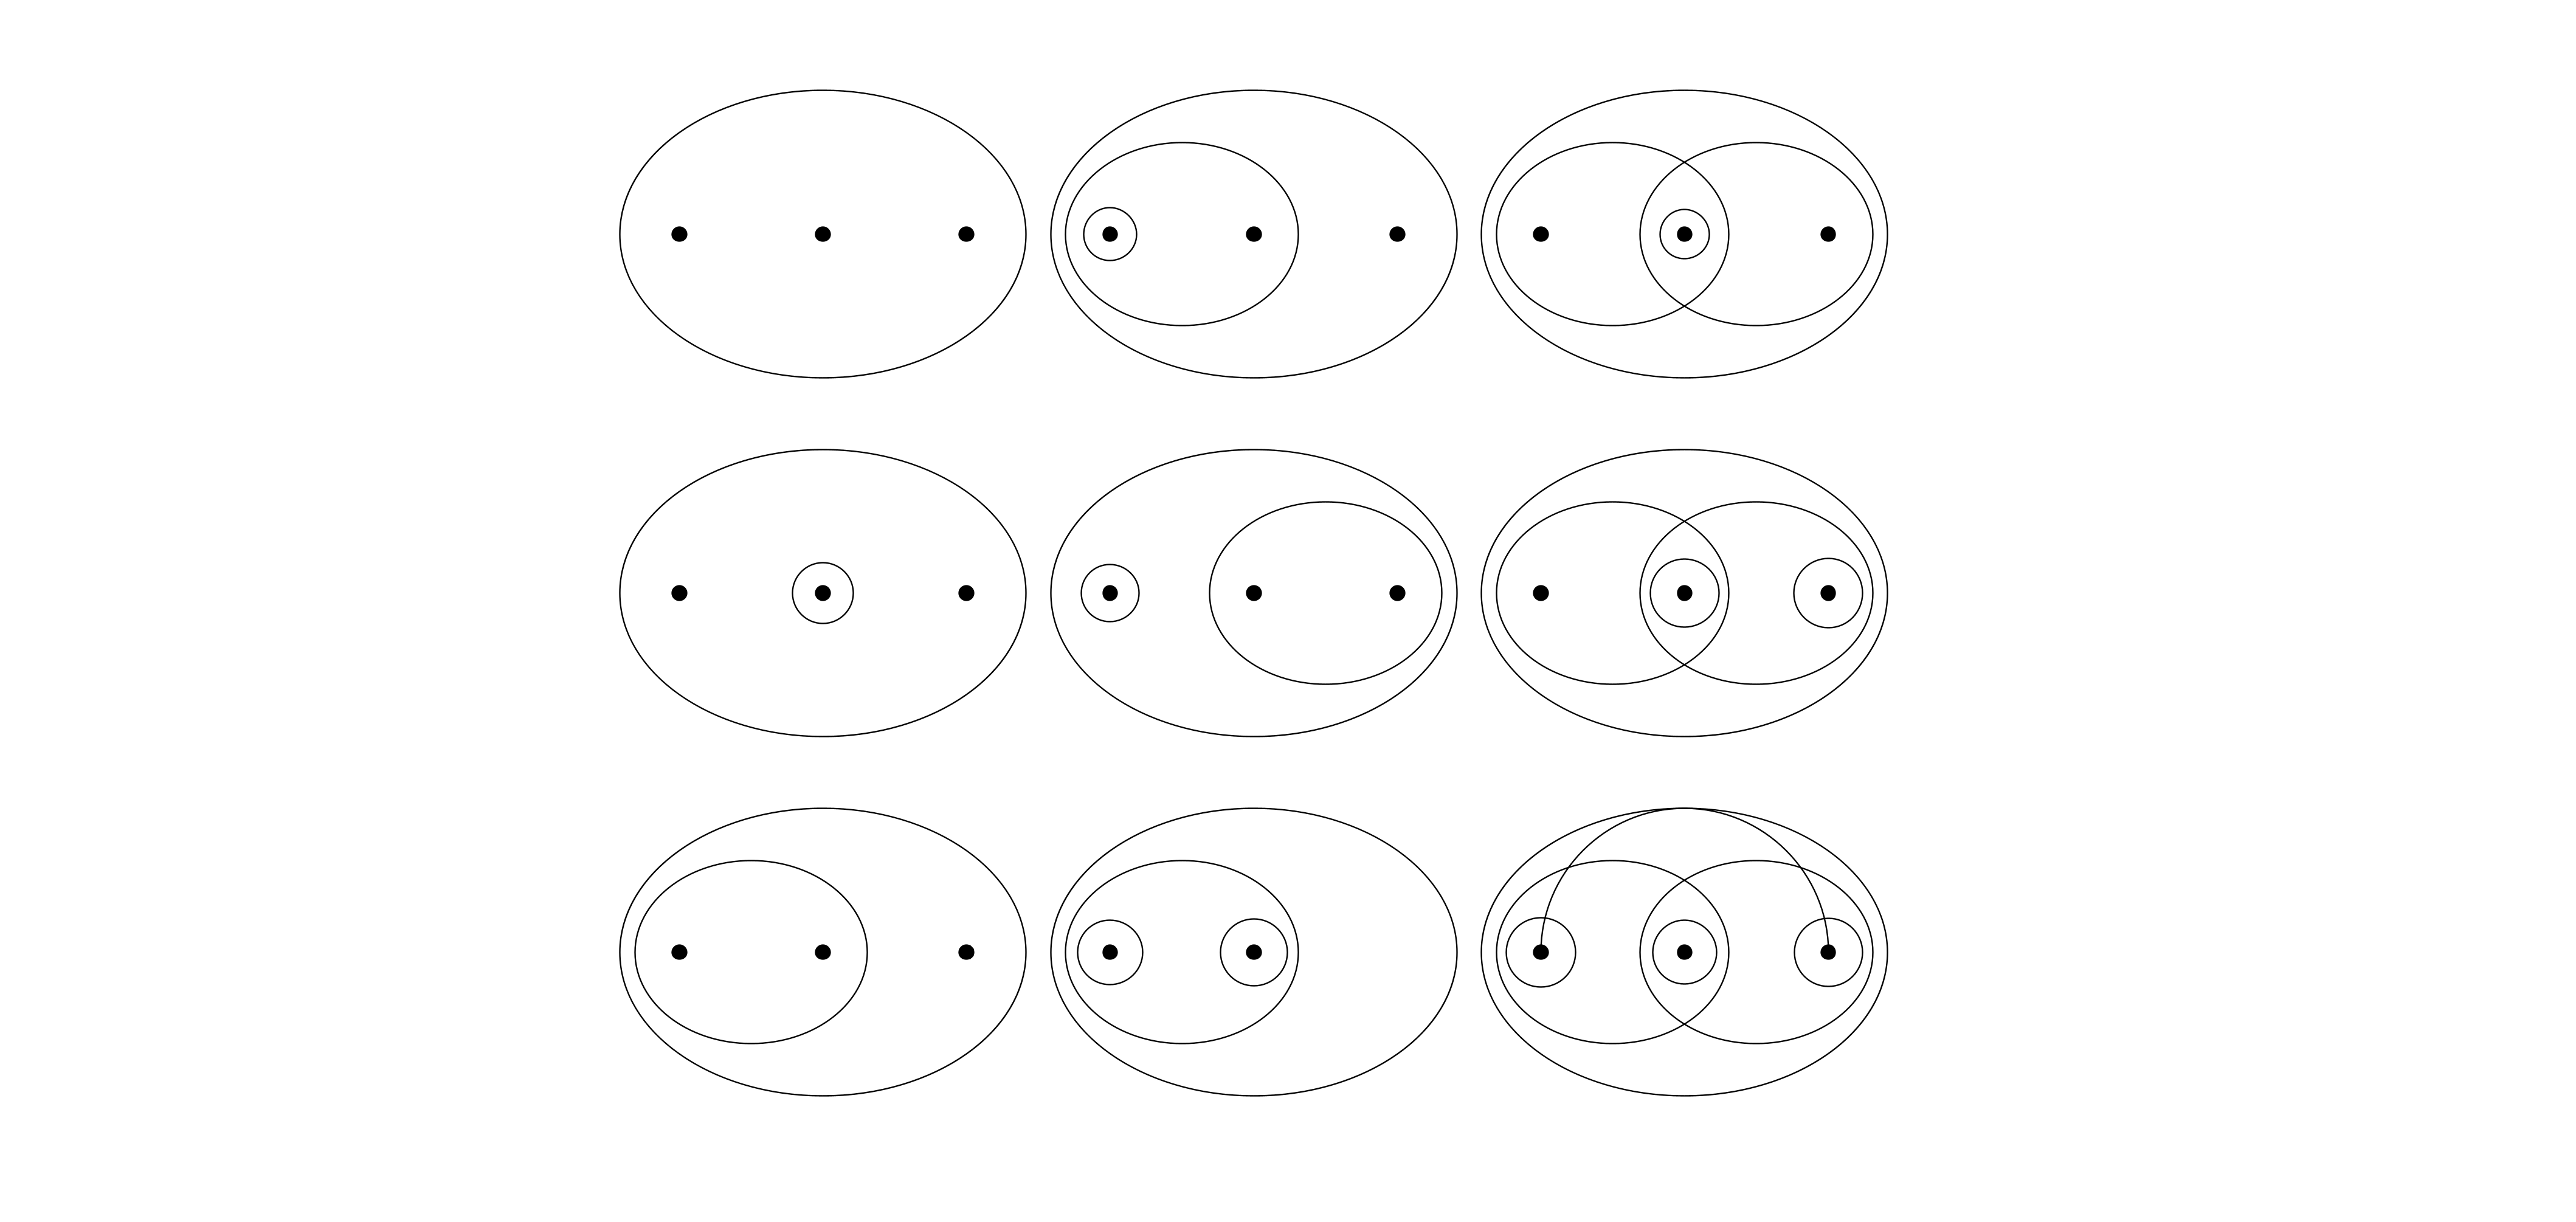
\includegraphics[scale = 0.3]{Figures/Chapter1/topologiesOn3Points.png}
                \caption{The Topologies on $\{a, b, c\}$.}
                \label{fig1.1}
            \end{figure}

        \item Let $X$ be any set, and let  $\Tc_f=\{U \subseteq X: \com{X}{U} \text{ is 
            finite, or } \com{X}{U}=X\}$. Then  $\Tc_f$ is a topology and called the 
            \textbf{finite complement topology}.

        \item Let $X$ be any set, and let  $\Tc_c=\{U \subseteq X: \com{X}{U} \text{ is 
            countable, or } \com{X}{U}=X\}$. Then  $\Tc_c$ is a topology on $X$.
    \end{enumerate}		
\end{example}

\begin{definition}
    Let $X$ be a set, and let $\Tc$ and  $\Tc'$ be topologies on  $X$. We say that 
    $\Tc$ is  \textbf{coarser} than $\Tc'$, and $\Tc'$ \textbf{finer} than $\Tc$ if  $\Tc \subseteq \Tc'$. 
    If two topologies are either coarser, or finer than each other, we call them \textbf{comparable}.
\end{definition}

\begin{example}
    The topologies $\Tc_f$ and  $\Tc_c$ are comparable, and we see that  $\Tc_f \subseteq \Tc_f$, so 
    $\Tc_f$ is coarser than  $\Tc_c$, and  $\Tc_c$ is finer than  $\Tc_f$.
\end{example} 
